\documentclass[letterpaper]{article} % DO NOT CHANGE THIS
\usepackage[submission]{aaai2027}  % DO NOT CHANGE THIS
% The serif, sans-serif, and monospaced fonts are loaded automatically by
% aaai2027.sty (newtxtext, helvet, courier). DO NOT add \usepackage{times},
% \usepackage{helvet}, \usepackage{courier}, or any other font package.
\usepackage[hyphens]{url}  % DO NOT CHANGE THIS
\usepackage{graphicx} % DO NOT CHANGE THIS
\urlstyle{rm} % DO NOT CHANGE THIS
\def\UrlFont{\rm}  % DO NOT CHANGE THIS
\usepackage{natbib}  % DO NOT CHANGE THIS AND DO NOT ADD ANY OPTIONS TO IT
\usepackage{caption} % DO NOT CHANGE THIS AND DO NOT ADD ANY OPTIONS TO IT
\frenchspacing  % DO NOT CHANGE THIS
%
% These are recommended to typeset algorithms but not required. See the subsubsection on algorithms. Remove them if you don't have algorithms in your paper.
\usepackage{algorithm}
\usepackage{algorithmic}

%
% These are recommended to typeset listings but not required. See the subsubsection on listing. Remove this block if you don't have listings in your paper.
\usepackage{newfloat}
\usepackage{listings}
\DeclareCaptionStyle{ruled}{labelfont=normalfont,labelsep=colon,strut=off} % DO NOT CHANGE THIS
\lstset{%
	basicstyle={\footnotesize\ttfamily},% footnotesize acceptable for monospace
	numbers=left,numberstyle=\footnotesize,xleftmargin=2em,% show line numbers, remove this entire line if you don't want the numbers.
	aboveskip=0pt,belowskip=0pt,%
	showstringspaces=false,tabsize=2,breaklines=true}
\floatstyle{ruled}
\newfloat{listing}{tb}{lst}{}
\floatname{listing}{Listing}

%
% Recommended for better-looking tables
\usepackage{booktabs}

%
% Keep the \pdfinfo as shown here. There's no need
% for you to add the /Title and /Author tags.
\pdfinfo{
/TemplateVersion (2027.1)
}

% DISALLOWED PACKAGES
% \usepackage{authblk} -- This package is specifically forbidden
% \usepackage{balance} -- This package is specifically forbidden
% \usepackage{CJK} -- This package is specifically forbidden
% \usepackage{float} -- This package is specifically forbidden
% \usepackage{flushend} -- This package is specifically forbidden
% \usepackage{fullpage} -- This package is specifically forbidden
% \usepackage{geometry} -- This package is specifically forbidden
% \usepackage{hyperref} -- This package is specifically forbidden
% \usepackage{navigator} -- This package is specifically forbidden
% (or any other package that embeds links such as navigator or hyperref)
% \usepackage{indentfirst} -- This package is specifically forbidden
% \usepackage{layout} -- This package is specifically forbidden
% \usepackage{multicol} -- This package is specifically forbidden
% \usepackage{nameref} -- This package is specifically forbidden
% \usepackage{savetrees} -- This package is specifically forbidden
% \usepackage{setspace} -- This package is specifically forbidden
% \usepackage{stfloats} -- This package is specifically forbidden
% \usepackage{tabu} -- This package is specifically forbidden
% \usepackage{titlesec} -- This package is specifically forbidden
% \usepackage{tocbibind} -- This package is specifically forbidden
% \usepackage{ulem} -- This package is specifically forbidden
% \usepackage{wrapfig} -- This package is specifically forbidden
% DISALLOWED COMMANDS
% \nocopyright -- Your paper will not be published if you use this command
% \addtolength -- This command may not be used
% \balance -- This command may not be used
% \baselinestretch -- Your paper will not be published if you use this command
% \clearpage -- No page breaks of any kind may be used for the final version of your paper
% \columnsep -- This command may not be used
% \newpage -- No page breaks of any kind may be used for the final version of your paper
% \pagebreak -- No page breaks of any kind may be used for the final version of your paper
% \pagestyle -- This command may not be used
% \tiny -- This is not an acceptable font size.
% \vspace{- -- No negative value may be used in proximity of a caption, figure, table, section, subsection, subsubsection, or reference
% \vskip{- -- No negative value may be used to alter spacing above or below a caption, figure, table, section, subsection, subsubsection, or reference

\setcounter{secnumdepth}{0} %May be changed to 1 or 2 if section numbers are desired.

% The file aaai2027.sty is the style file for AAAI Press
% proceedings, working notes, and technical reports.
%

% Title

% Your title must be in mixed case, not sentence case.
% That means all verbs (including short verbs like be, is, using,and go),
% nouns, adverbs, adjectives should be capitalized, including both words in hyphenated terms, while
% articles, conjunctions, and prepositions are lower case unless they
% directly follow a colon or long dash
\title{FinOKF: Evidence-Aware Finance Open Knowledge Formatting with LRU Caching for Auditable Equity Research}
\author{Anonymous Submission}
\affiliations{}
\begin{document}
\maketitle

\begin{abstract}
Equity-research answers must be numerically correct, traceable, and economical to produce. FinOKF separates measurement validation and deterministic arithmetic from language-model interpretation, using an evidence-dependent LRU cache and inspectable knowledge graphs. We audit 42 saved agent records across GPT-5.5, Claude Sonnet 5, and Llama 3.2 3B on seven questions. A retrospective margin panel contains 37 entries per model, representing 15 distinct measurements. FinOKF correctly reports 37, 34, and 32 entries respectively; the corresponding web baselines correctly report 22, 4, and 0. These counts distinguish omissions, conflicting periods, and execution failures, and do not score every narrative claim. The wider audit finds that correct calculation tables can coexist with erroneous interpretations in Claude and Llama responses. Over 16 pairs with successful execution status, FinOKF reduces mean tokens by 90.9--97.1\%, with baseline-to-FinOKF mean latency ratios of 6.9--15.8. The results support lower workflow cost and better coverage of the audited measurements, while showing that validated evidence does not guarantee faithful synthesis. Unequal completion, retrospective scoring, and predominantly warm caching limit generalization and causal attribution.
\end{abstract}

\section{Introduction}
An analyst assessing whether growth is becoming more profitable must identify the issuer, select comparable reporting periods, distinguish consolidated and segment values, normalize units, and calculate the relevant change. A plausible narrative cannot repair an incorrect input or denominator. Repeatedly asking a language model to reconstruct these relationships also repeats retrieval and computation.

Financial question answering therefore requires both numerical evidence and contextual interpretation \citep{chen2021finqa,zhu2021tatqa}. FinOKF addresses this requirement with a simple execution policy: resolve the company in Python, retrieve local evidence, validate financial measurements, perform supported arithmetic, reuse intermediate evidence when valid, and request fresh model synthesis. The research question is whether measurement-aware preprocessing and LRU caching can reduce resource consumption while retaining useful, correct equity-research outputs.

The mechanisms are distinct. Validation and deterministic arithmetic protect supported numerical operations; compact evidence reduces context; caching can avoid repeated preparation and research. Caching itself does not improve model reasoning. This paper contributes an implemented integration of these mechanisms, a corpus and conversation graph for inspection, and a reproducible retrospective audit of saved GPT-5.5, Claude Sonnet 5, and Llama 3.2 3B answers. We report correctness conditional on an answer being supplied separately from measurement coverage and abstention. This prevents a missing answer from being mislabeled as a fabricated number, while exposing a practical limitation of repeated web research.

\section{Related Work}
FinQA represents financial answers as reasoning programs over reports \citep{chen2021finqa}; TAT-QA combines tabular and textual evidence \citep{zhu2021tatqa}. They motivate explicit numerical reasoning but are not benchmarks evaluated here. Retrieval-augmented generation supplies external evidence to a model \citep{lewis2020rag}; retrieval alone does not establish that selected measurements have compatible periods or scales. Program-aided language models delegate generated computations to an interpreter \citep{gao2023pal}. FinOKF instead uses predefined financial operations with bounded eligibility rules.

SEC EDGAR APIs provide submissions and XBRL facts \citep{secapi}, while XBRL specifies structured reporting concepts and contexts \citep{xbrl2026standard}. Recency-based caching has a long history in database buffering \citep{oneil1993lruk}. FinOKF contributes their integration into an inspectable analyst workflow, rather than a new replacement algorithm or a general financial reasoning engine.

\section{System and Measurement Contract}
The pipeline comprises ingestion, preprocessing, entity resolution, evidence preparation and reuse, and answer persistence. Local SEC filings, company facts, submissions, and downloaded Yahoo Finance prices form the evidence corpus. The present evaluation uses annual filing measurements for Microsoft and Apple; it does not evaluate price analysis. Figure~\ref{fig:flowchart} depicts the supplied deployment overview.

\begin{figure}[t]
\centering
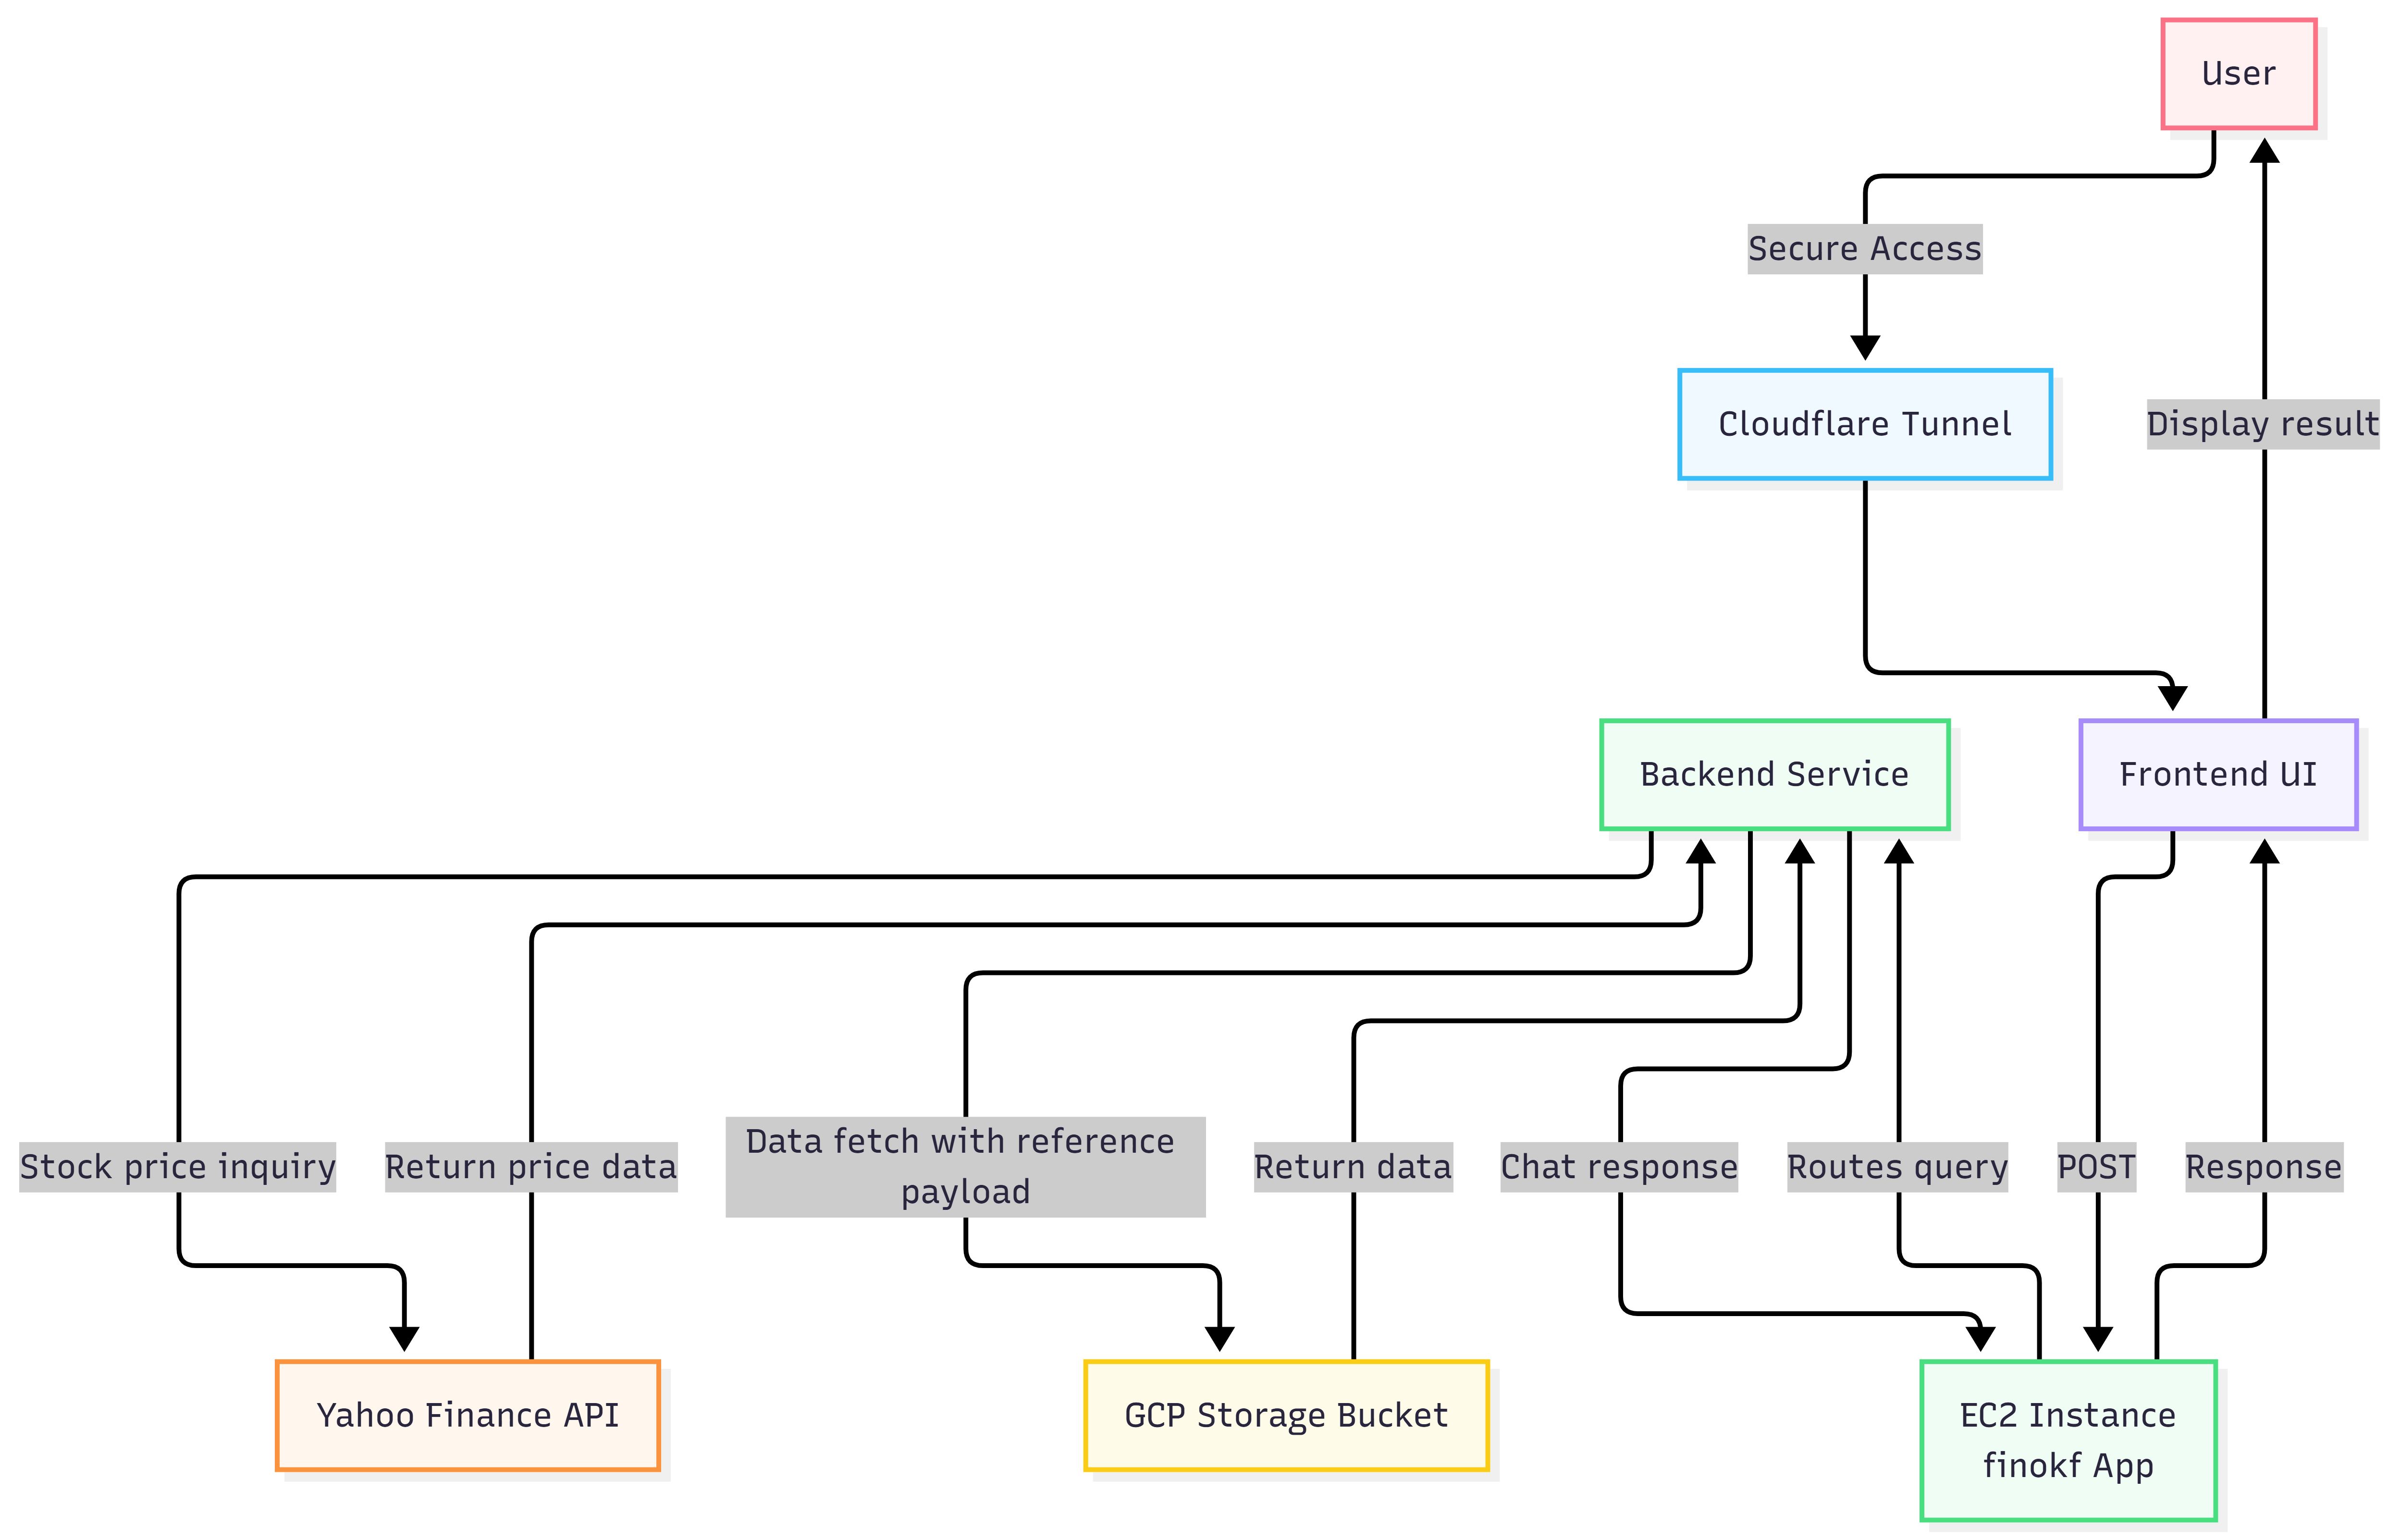
\includegraphics[width=\columnwidth]{../assets/flowchart.png}
\caption{Supplied deployment overview linking the frontend, backend, compute service, storage, and price-retrieval service.}
\label{fig:flowchart}
\end{figure}

\subsection{Validated Measurements}
Preprocessing repairs malformed Markdown tables and represents declared magnitudes explicitly, accounting for exceptions such as percentages and per-share quantities. A measurement is
\begin{equation}
m=(c,v,s,u,\gamma,p,d,\ell),\qquad x(m)=v\,s,
\end{equation}
where $c$ is concept, $v$ stored value, $s$ multiplier, $u$ unit, $\gamma$ currency, $p$ reporting period, $d$ dimensions, and $\ell$ source location. The period includes fiscal year, exact dates, and duration or instant kind. An already normalized dollar amount has multiplier one.

The annual calculation path selects recognized financial concepts, requires consolidated duration facts with empty dimensions, checks matching periods, and rejects conflicting candidates. Its operational annual-duration window is 350--380 days. Monetary inputs must be finite and denominated in USD. Unsupported concepts, missing years, incompatible units, and ambiguous bindings fall through to broader research. Table repair and validation are not guarantees of complete or error-free extraction.

For validated revenue $R_t$, cost of revenue $C_t$, and operating income $O_t$, the audited metrics are
\begin{equation}
\mathrm{GM}_t=\frac{R_t-C_t}{R_t},\qquad
\mathrm{OM}_t=\frac{O_t}{R_t},
\end{equation}
\begin{equation}
\mathrm{IOM}_{a,b}=\frac{O_b-O_a}{R_b-R_a}.
\end{equation}
Margins are displayed as percentages. The basis-point change is $10^4(M_b-M_a)$ for a fractional margin $M$. Zero revenue change makes IOM undefined; ordinary margins are not reported for nonpositive revenue. Supported operations also include net margin and cash conversion, but those are outside the evaluated workload.

\subsection{Routing and Evidence Compression}
Python identifies company names and tickers before invoking the model and limits eligible nodes to the resolved company set. Explicit company mentions in a new question determine the retrieval scope independently of earlier turns. Local filing selection and prompt budgets then determine supplied evidence; graph neighbors cannot bypass the ticker allowlist.

Supported calculations yield compact tables of validated inputs, results, periods, and source paths. The selected model generates an interpretation from this evidence, including on a cache hit. Unsupported requests use broader local retrieval and, when coverage is insufficient, supplementary web research. A compact ratio package supports measured trends but cannot by itself establish management intent, segment drivers, causality, or future persistence.

\subsection{Evidence Reuse}
An in-memory, lock-protected LRU defaults to 128 entries. Access updates recency, capacity overflow evicts the least recently used entry, and returned objects are deep copies. Capacity zero disables caching; process restart clears it.

The annual calculation key is $H(e,o,Y,B)$: ticker, recognized operation, requested fiscal years, and serialized measurement bindings. Changed values, scales, units, periods, or included source metadata change the key. Model and provider are absent because this object is numerical evidence. The implementation still selects bindings, validates them, and computes per-year ratios before lookup; a hit does not eliminate all arithmetic. It also does not independently hash every byte of every filing at request time.

Research keys include provider, model, endpoint, method, and prompts containing local evidence. Entries expire after 900 seconds, or 60 seconds when retrieval warnings occur. This is wording-sensitive reuse, not a general semantic paraphrase cache. A hit can skip coverage assessment and external retrieval, but fresh final synthesis still incurs model latency and tokens. The evaluated records exercise calculation caching only.

\begin{figure}[t]
\centering
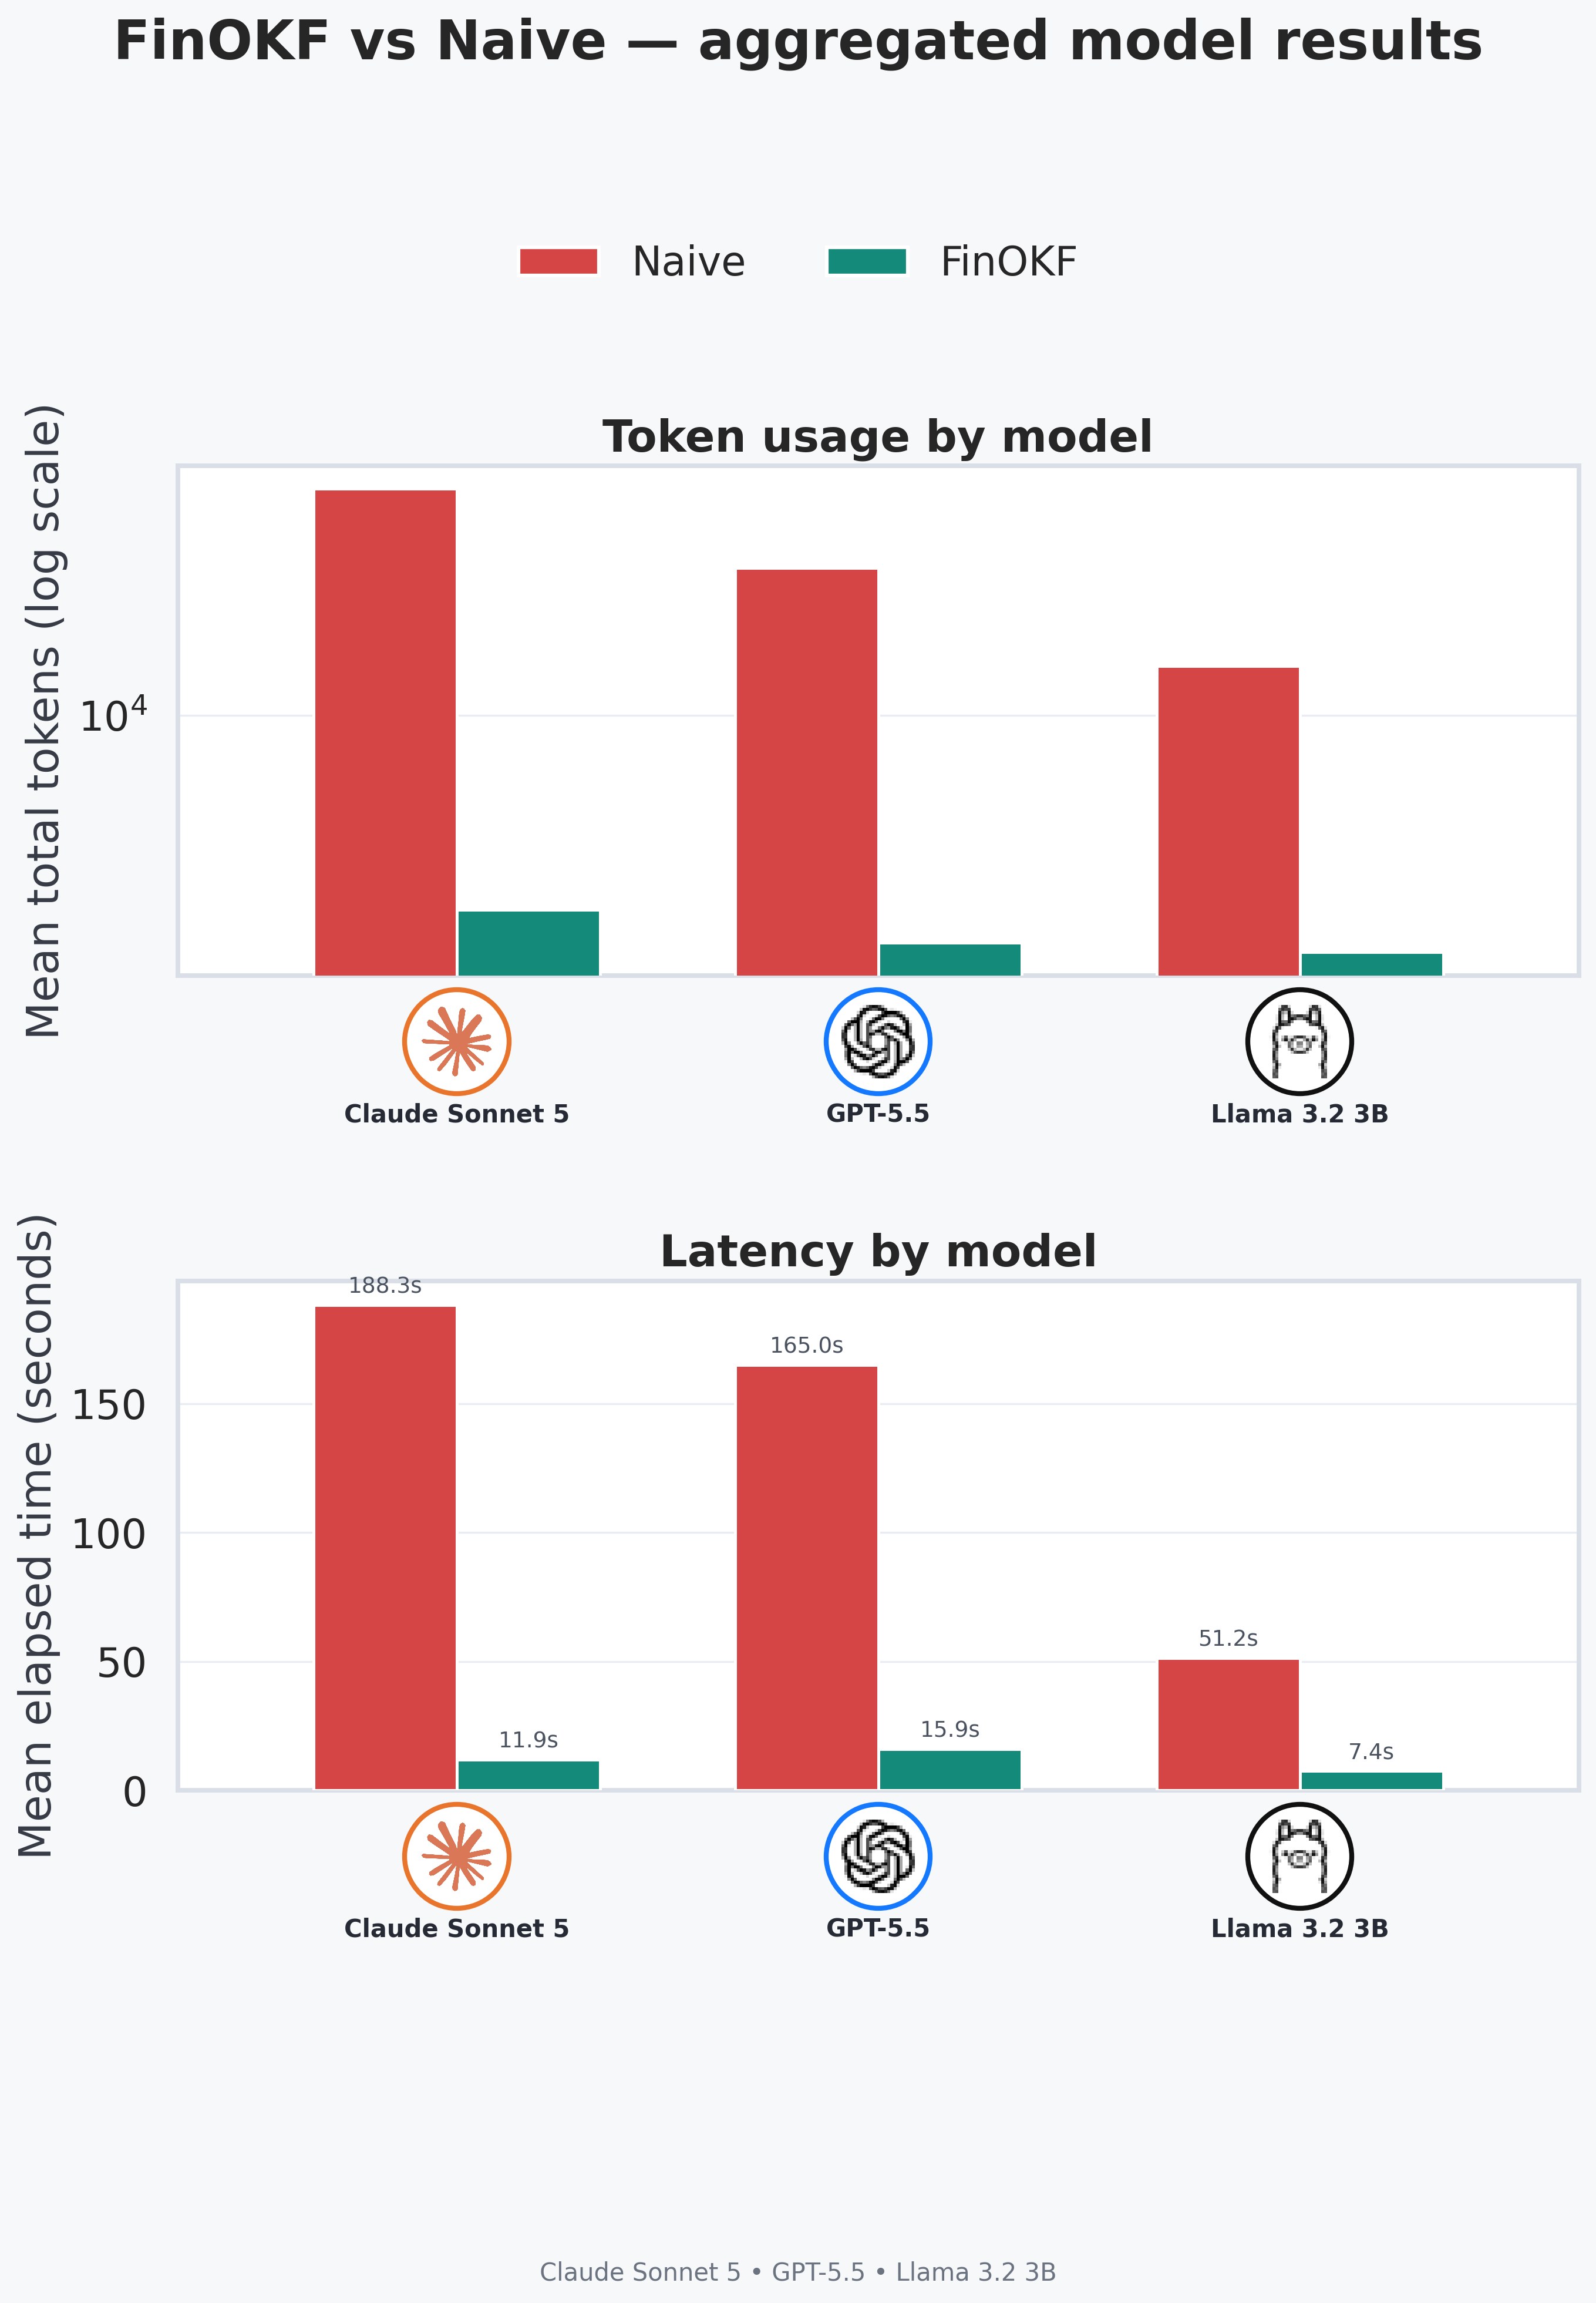
\includegraphics[width=0.92\columnwidth,height=0.42\textheight,keepaspectratio]{../assets/model_results_vertical.png}
\caption{Paired means for GPT-5.5, Claude Sonnet 5, and Llama 3.2 3B. Tokens aggregate completed calls; latency includes the full workflow.}
\label{fig:models}
\end{figure}

\section{Knowledge Graph and Provenance}
FinOKF maintains complementary corpus and conversation graphs. Nodes have identifiers, types, and paths to inspectable files; edges record document membership or execution relationships.

\subsection{Corpus Graph}
The index builder creates a \texttt{finance.entity} company hub per ticker and \texttt{finance.filing} nodes carrying form, accession, filing date, reporting date, and available fiscal-year metadata. Company-to-filing \texttt{has\_filing} edges have reciprocal \texttt{filed\_by} edges. Within a company, filing-date/accession ordering supplies \texttt{prior\_filing} and \texttt{next\_filing} links; available \texttt{amends} links are preserved.

The browser overview displays companies, filings, and membership links (Figure~\ref{fig:knowledge-graph}). It omits individual fact nodes and does not draw the stored temporal links. Layout positions group filings by ticker; spacing does not encode economic relationships or semantic similarity. Colors distinguish filing forms, and node selection opens the associated document. Navigability establishes document association, while the separate measurement contract establishes eligibility for arithmetic.

\begin{figure}[t]
\centering
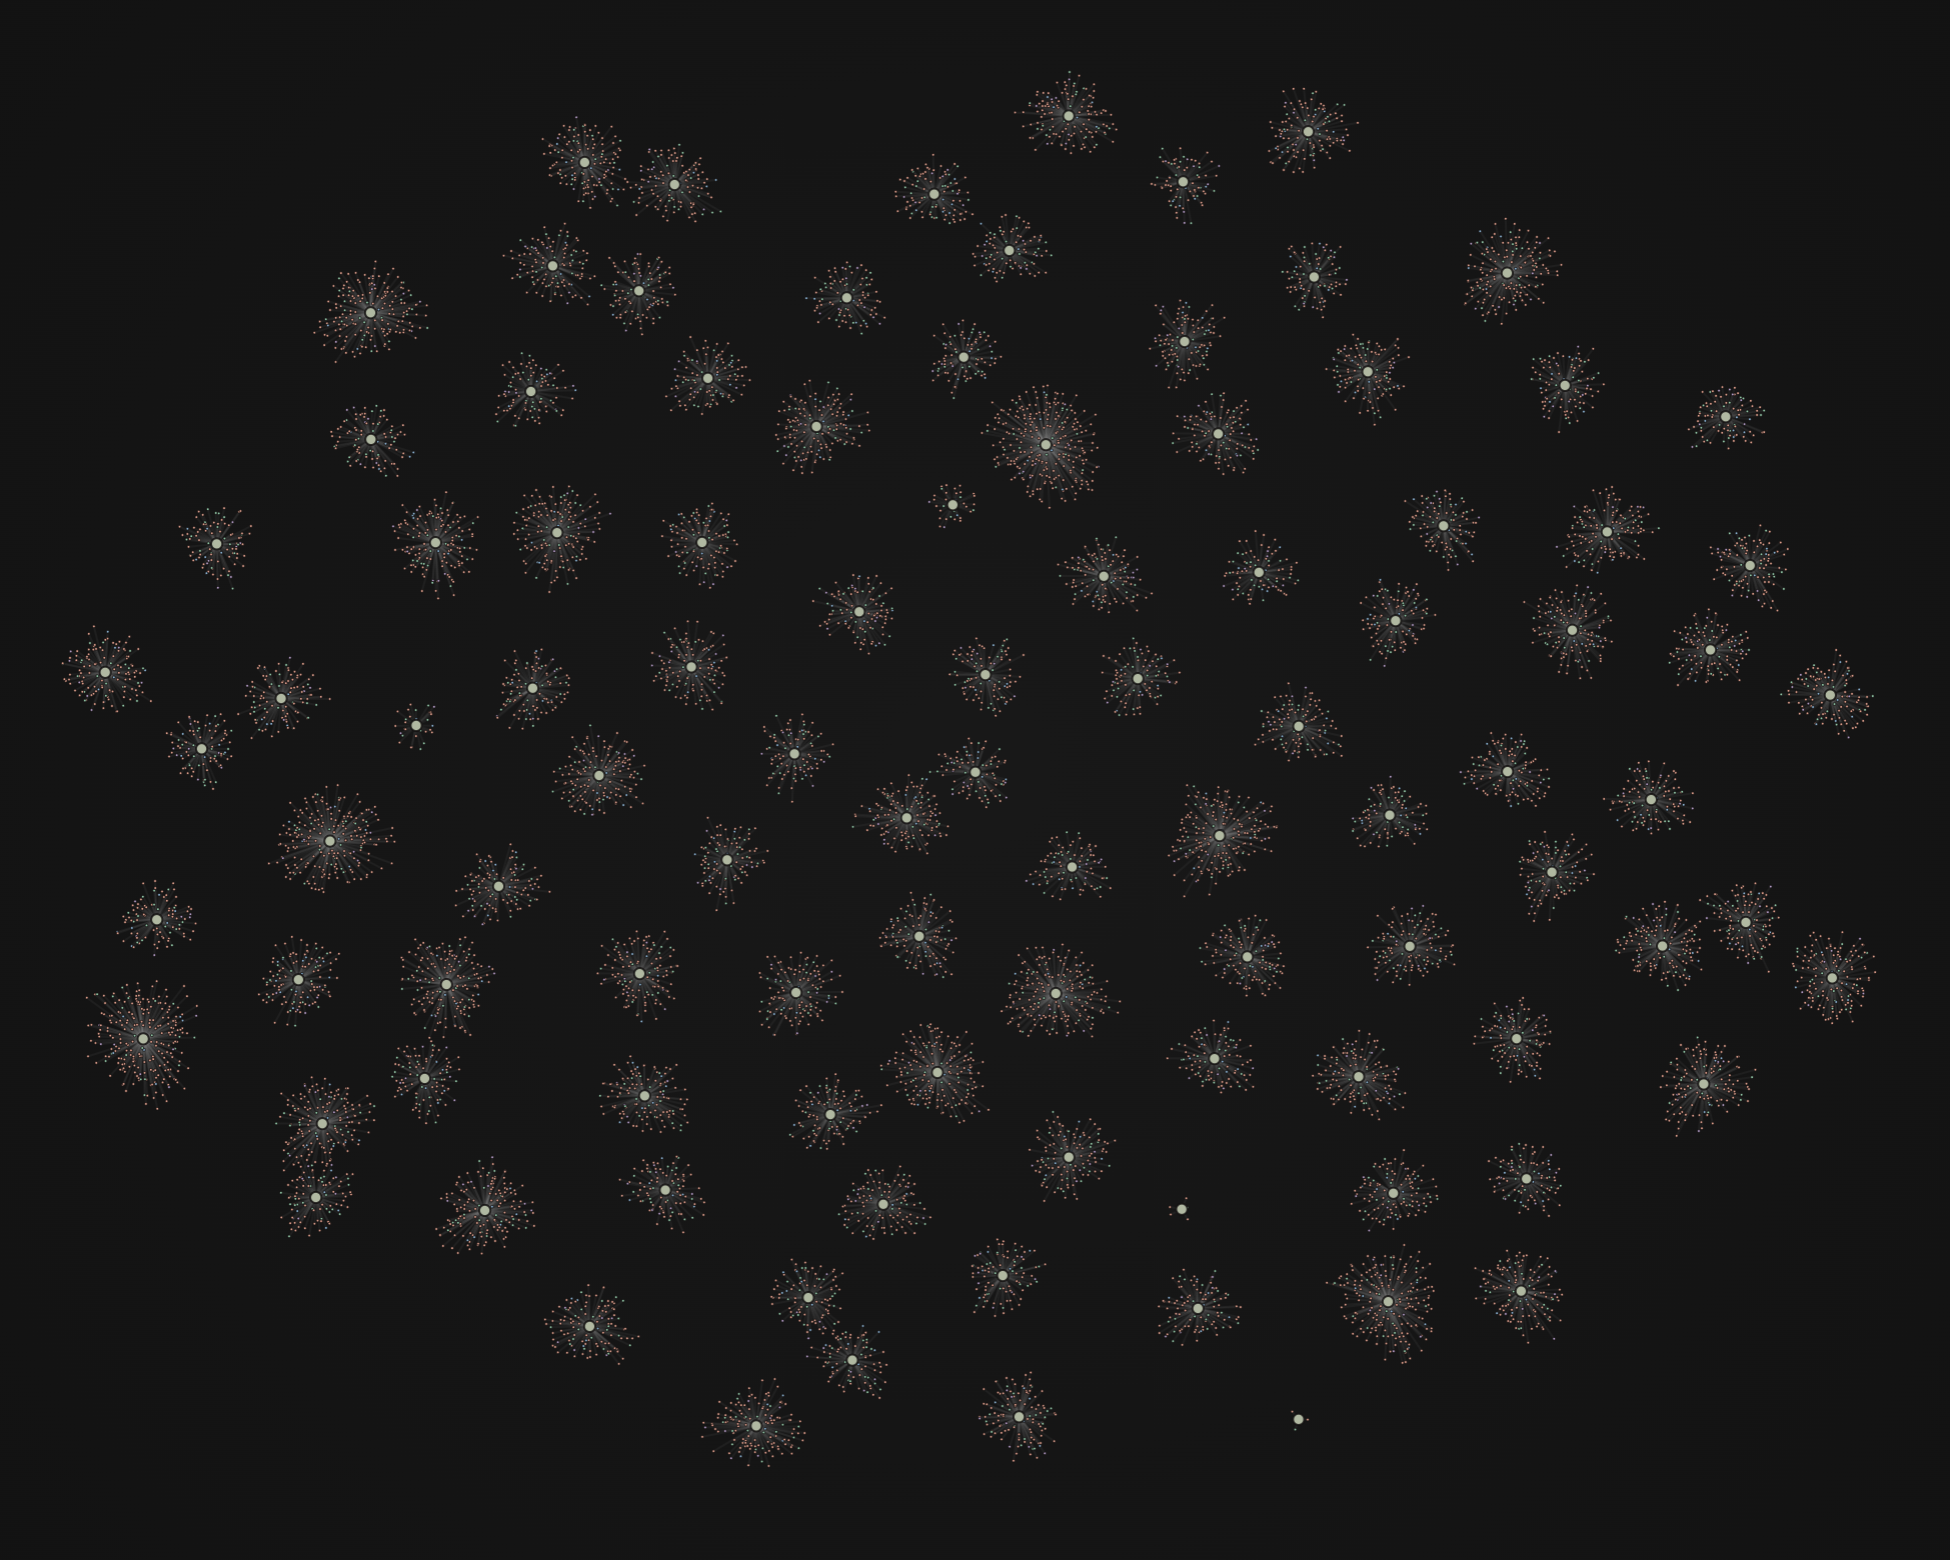
\includegraphics[width=\columnwidth]{../assets/knowledge_graph.png}
\caption{Supplied corpus graph: pale-green company hubs and surrounding filings. Colors distinguish 10-K (blue), 10-Q (green), 8-K (salmon), DEF 14A (purple), and other forms (neutral). Spatial distance is a layout choice.}
\label{fig:knowledge-graph}
\end{figure}

\subsection{Conversation Graph and Vault}
Each turn adds an execution and a durable answer node. A vault \texttt{executes} a run; a run \texttt{produces} an answer and \texttt{binds} or \texttt{reuses} recorded evidence according to its cache-hit flag. The cumulative graph merges turns, deduplicates typed links, and associates ticker-tagged nodes with companies using \texttt{has\_evidence}. It does not import unused corpus neighbors. A \texttt{reuses} edge denotes the execution's recorded state, not proof of a separate cache lookup for every linked item.

Vaults retain questions, answers, bindings, execution metrics, and source snapshots. Local sources are copied byte-for-byte; altered content receives a versioned copy. This preserves the selected local Markdown, not the original SEC HTML. Per-turn snapshots preserve history while the cumulative graph deduplicates logical sources. Web excerpts and generated notes are identified as generated evidence. Prompt-budget exclusions are omitted from the turn's evidence record.

Answer nodes preserve the available provider, model, route, source, and cost metadata. Unavailable usage is not represented as zero. Provenance makes supplied evidence inspectable, but does not expose private model reasoning or establish that every narrative assertion follows from its citations.

\section{Three-Model Evaluation}
\subsection{Records and Comparison}
We inspect all six saved vaults for GPT-5.5 (\texttt{gpt-5.5}), Claude Sonnet 5 (\texttt{claude-sonnet-5}), and Llama 3.2 3B (\texttt{llama3.2:3b}), dated September 8, 2026. Each configuration has seven FinOKF and seven Naive result records: 42 attempts in total. The recorded identifiers are reported verbatim. Three questions concern Microsoft's FY2023--FY2025 operating leverage, including a paraphrase and a narrowed FY2024--FY2025 follow-up. Three similarly examine Apple's gross margin; the seventh compares both companies' operating leverage. We apply the same question-level audit panel to all three configurations.

For each question, Naive starts independent web research without local filings, prices, vaults, or application cache. FinOKF uses validated local calculation evidence. All 21 FinOKF executions have successful status. Naive has seven successful statuses for GPT-5.5, seven for Llama, and two for Claude; five Claude records explicitly report no text output. Both successful Claude baseline answers also end mid-calculation or mid-sentence. We audit the text actually saved and do not equate successful execution status with a complete or correct answer.

Resource comparisons use 16 matched successful-status pairs: seven GPT, seven Llama, and Claude Questions 2.1 and 2.3. Each paired Naive run has three completed model calls; each FinOKF run has one. FinOKF cache hits number 7/7 for GPT, 7/7 for Claude, and 3/7 for Llama; 12/16 matched FinOKF runs are hits. These are not controlled cold-start trials. Agents run concurrently with different research and response budgets. There is one saved run per condition, without independent repetitions.

\subsection{Accuracy and Consistency Method}
We recompute reference values from consolidated statement rows in the vault copies of the Microsoft and Apple FY2025 10-Ks, cross-checked against issuer publications \citep{msft2025report,apple2025results,apple2024results}. A standalone audit uses Decimal arithmetic without importing FinOKF's calculation helpers or using generated bindings as the reference.

The fixed panel covers annual margin levels, annual margin changes, and incremental operating margins: 7, 7, 4, 5, 5, 3, and 6 entries for Questions 1.1--2.4. Each model therefore has 37 entries, containing 15 distinct company--metric--period values reused across follow-ups. The six model--agent conditions yield 222 audit records. An entry is reported only when explicitly supplied; values a reader could calculate remain omitted.

The tolerance is half the last displayed unit after unit conversion. A correctly rounded value assigned to the wrong period fails. Conflicting prose and table period assignments are marked inconsistent rather than crediting only the correct occurrence. Repeated consistent mentions count once. No-text execution failures are unavailable, separate from omissions in returned text. We report correct entries, incorrect or inconsistent entries, omissions, and unavailable entries separately.

This is an agent-assisted retrospective annotation with reproducible arithmetic, not a blinded expert study or an exhaustive factuality score. The panel favors explicit margin reporting and does not exhaust valid formulations. Additional source, arithmetic, and interpretation defects are documented separately in the appendix and machine-readable audit. A high panel score cannot establish that the whole answer is accurate.

\begin{table}[t]
\centering
\begin{tabular}{llrrrr}
\toprule
Model & Agent & C & E & O & U\\
\midrule
GPT-5.5 & FinOKF & 37 & 0 & 0 & 0\\
 & Naive & 22 & 0 & 15 & 0\\
Claude Sonnet 5 & FinOKF & 34 & 0 & 3 & 0\\
 & Naive & 4 & 2 & 2 & 29\\
Llama 3.2 3B & FinOKF & 32 & 3 & 2 & 0\\
 & Naive & 0 & 1 & 36 & 0\\
\bottomrule
\end{tabular}
\caption{All-record retrospective margin panel, 37 entries per row. C: correct; E: incorrect or inconsistent; O: omitted in returned text; U: unavailable because execution failed. Llama FinOKF's E comprises one wrong value and two conflicting period assignments. These are panel counts, not whole-answer accuracy.}
\label{tab:accuracy}
\end{table}

\subsection{Results by Model}
\paragraph{GPT-5.5.}
FinOKF reports 37/37 correct panel entries; Naive reports 22/22 correctly and omits 15. Conditional panel correctness is 100\% for both, while coverage is 100\% versus 59.5\%. Naive explicitly abstains on Apple's repeated question (2.2); its Microsoft repeat (1.2) gives a valid qualitative conclusion from rounded growth rates but only one panel quantity. These are coverage differences, not fabricated numbers. FinOKF answers all seven questions quantitatively but omits an explicit different-fiscal-year-end caveat in the company comparison, which Naive includes.

\paragraph{Claude Sonnet 5.}
FinOKF reports 34/34 panel entries correctly and omits three margin levels in Question 1.2. The baseline's two returned texts supply six entries: four correct and two outside display-rounding tolerance. Question 2.1 states FY2025 gross margin as 46.90\% and its annual gain as approximately 69 bp, whereas unrounded references are 46.905164\% and 69.881429 bp. The remaining two entries in these returned texts are omitted; 29 entries are unavailable across five no-text failures. We do not treat those failures as 29 incorrect financial claims.

Despite correct panel entries, Claude FinOKF describes incremental margins falling from 62.97\% to 52.17\% as nearly halving, confuses proportional and absolute profit growth in another answer, and suggests an unsupported FY2026 margin assumption. Its company comparison visibly corrects an initial reversed inequality. Thus its panel correctness does not establish narrative reliability.

\paragraph{Llama 3.2 3B.}
FinOKF has 32 correct, one incorrect, two inconsistent, and two omitted entries: conditional panel correctness is 32/35 (91.4\%). In Question 1.2, the model assigns 52.17\% IOM to FY2024 instead of 62.97\%. In Apple's repeat, correct table intervals conflict with prose assigning both changes one year early. The baseline reports only one panel value, a wrong-period Microsoft margin; its other 36 entries are omitted. Zero correct panel entries must not be interpreted as zero correctness across every statement.

The narrative audit reveals further defects. FinOKF calls 45.62\% lower than 44.64\%, describes shrinking Apple margin gains as strengthening, invents supplementary growth rates, and labels an IOM formula as a margin-change formula. Llama Naive substitutes quarterly gross-profit dollars for annual analysis, presents \$48,341 million as 48.341\%, and supplies erroneous Microsoft operating income. These examples substantiate the risk that compact validated evidence can be copied correctly into a table yet interpreted incorrectly.

\subsection{Meaning of Accuracy and Provenance}
The audited references show Microsoft's IOM falling from 62.968651\% to 52.169280\%, and Apple's annual GM gains slowing from 207.522024 to 69.881429 bp. These are useful tests of trend direction as well as arithmetic. GPT's cross-company baseline uses a valid alternative: operating-income growth divided by revenue growth. This can favor Apple while IOM and margin expansion favor Microsoft; differing definitions are not automatically errors.

All 24 filing-source entries in FinOKF result metadata resolve to archived copies that match local documents by SHA-256. This verifies recorded source preservation, not that every prose citation is supported: some Llama answers additionally mention price files or unspecified CSV evidence outside the recorded sources. Microsoft's June 30 year-end and Apple's late-September year-end also mean the comparison is not over identical calendar windows. The appendix separates such caveats, self-corrections, unsupported drivers, and source defects from the fixed panel score.

\subsection{Resource Results}
Table~\ref{tab:cost} and Figure~\ref{fig:models} recompute mean costs over matched successful-status pairs. Reductions in mean total tokens are 95.7\% for GPT, 97.1\% for Claude, and 90.9\% for Llama. Baseline-to-FinOKF ratios of mean elapsed time are 10.4, 15.8, and 6.9. These are ratios, not millisecond measurements.

\begin{table}[t]
\centering
\begin{tabular}{lrrrrr}
\toprule
 & & \multicolumn{2}{c}{Mean tokens} & \multicolumn{2}{c}{Time (s)}\\
Model & $n$ & Naive & FinOKF & Naive & FinOKF\\
\midrule
GPT-5.5 & 7 & 34,475 & 1,487 & 165.0 & 15.9\\
Claude & 2 & 66,959 & 1,964 & 188.3 & 11.9\\
Llama & 7 & 15,138 & 1,375 & 51.2 & 7.4\\
\bottomrule
\end{tabular}
\caption{Paired successful-status cost means. Claude uses only Questions 2.1 and 2.3; other configurations use all seven. Unequal workloads and truncated baseline text prevent intrinsic model-performance rankings.}
\label{tab:cost}
\end{table}

\begin{figure}[t]
\centering
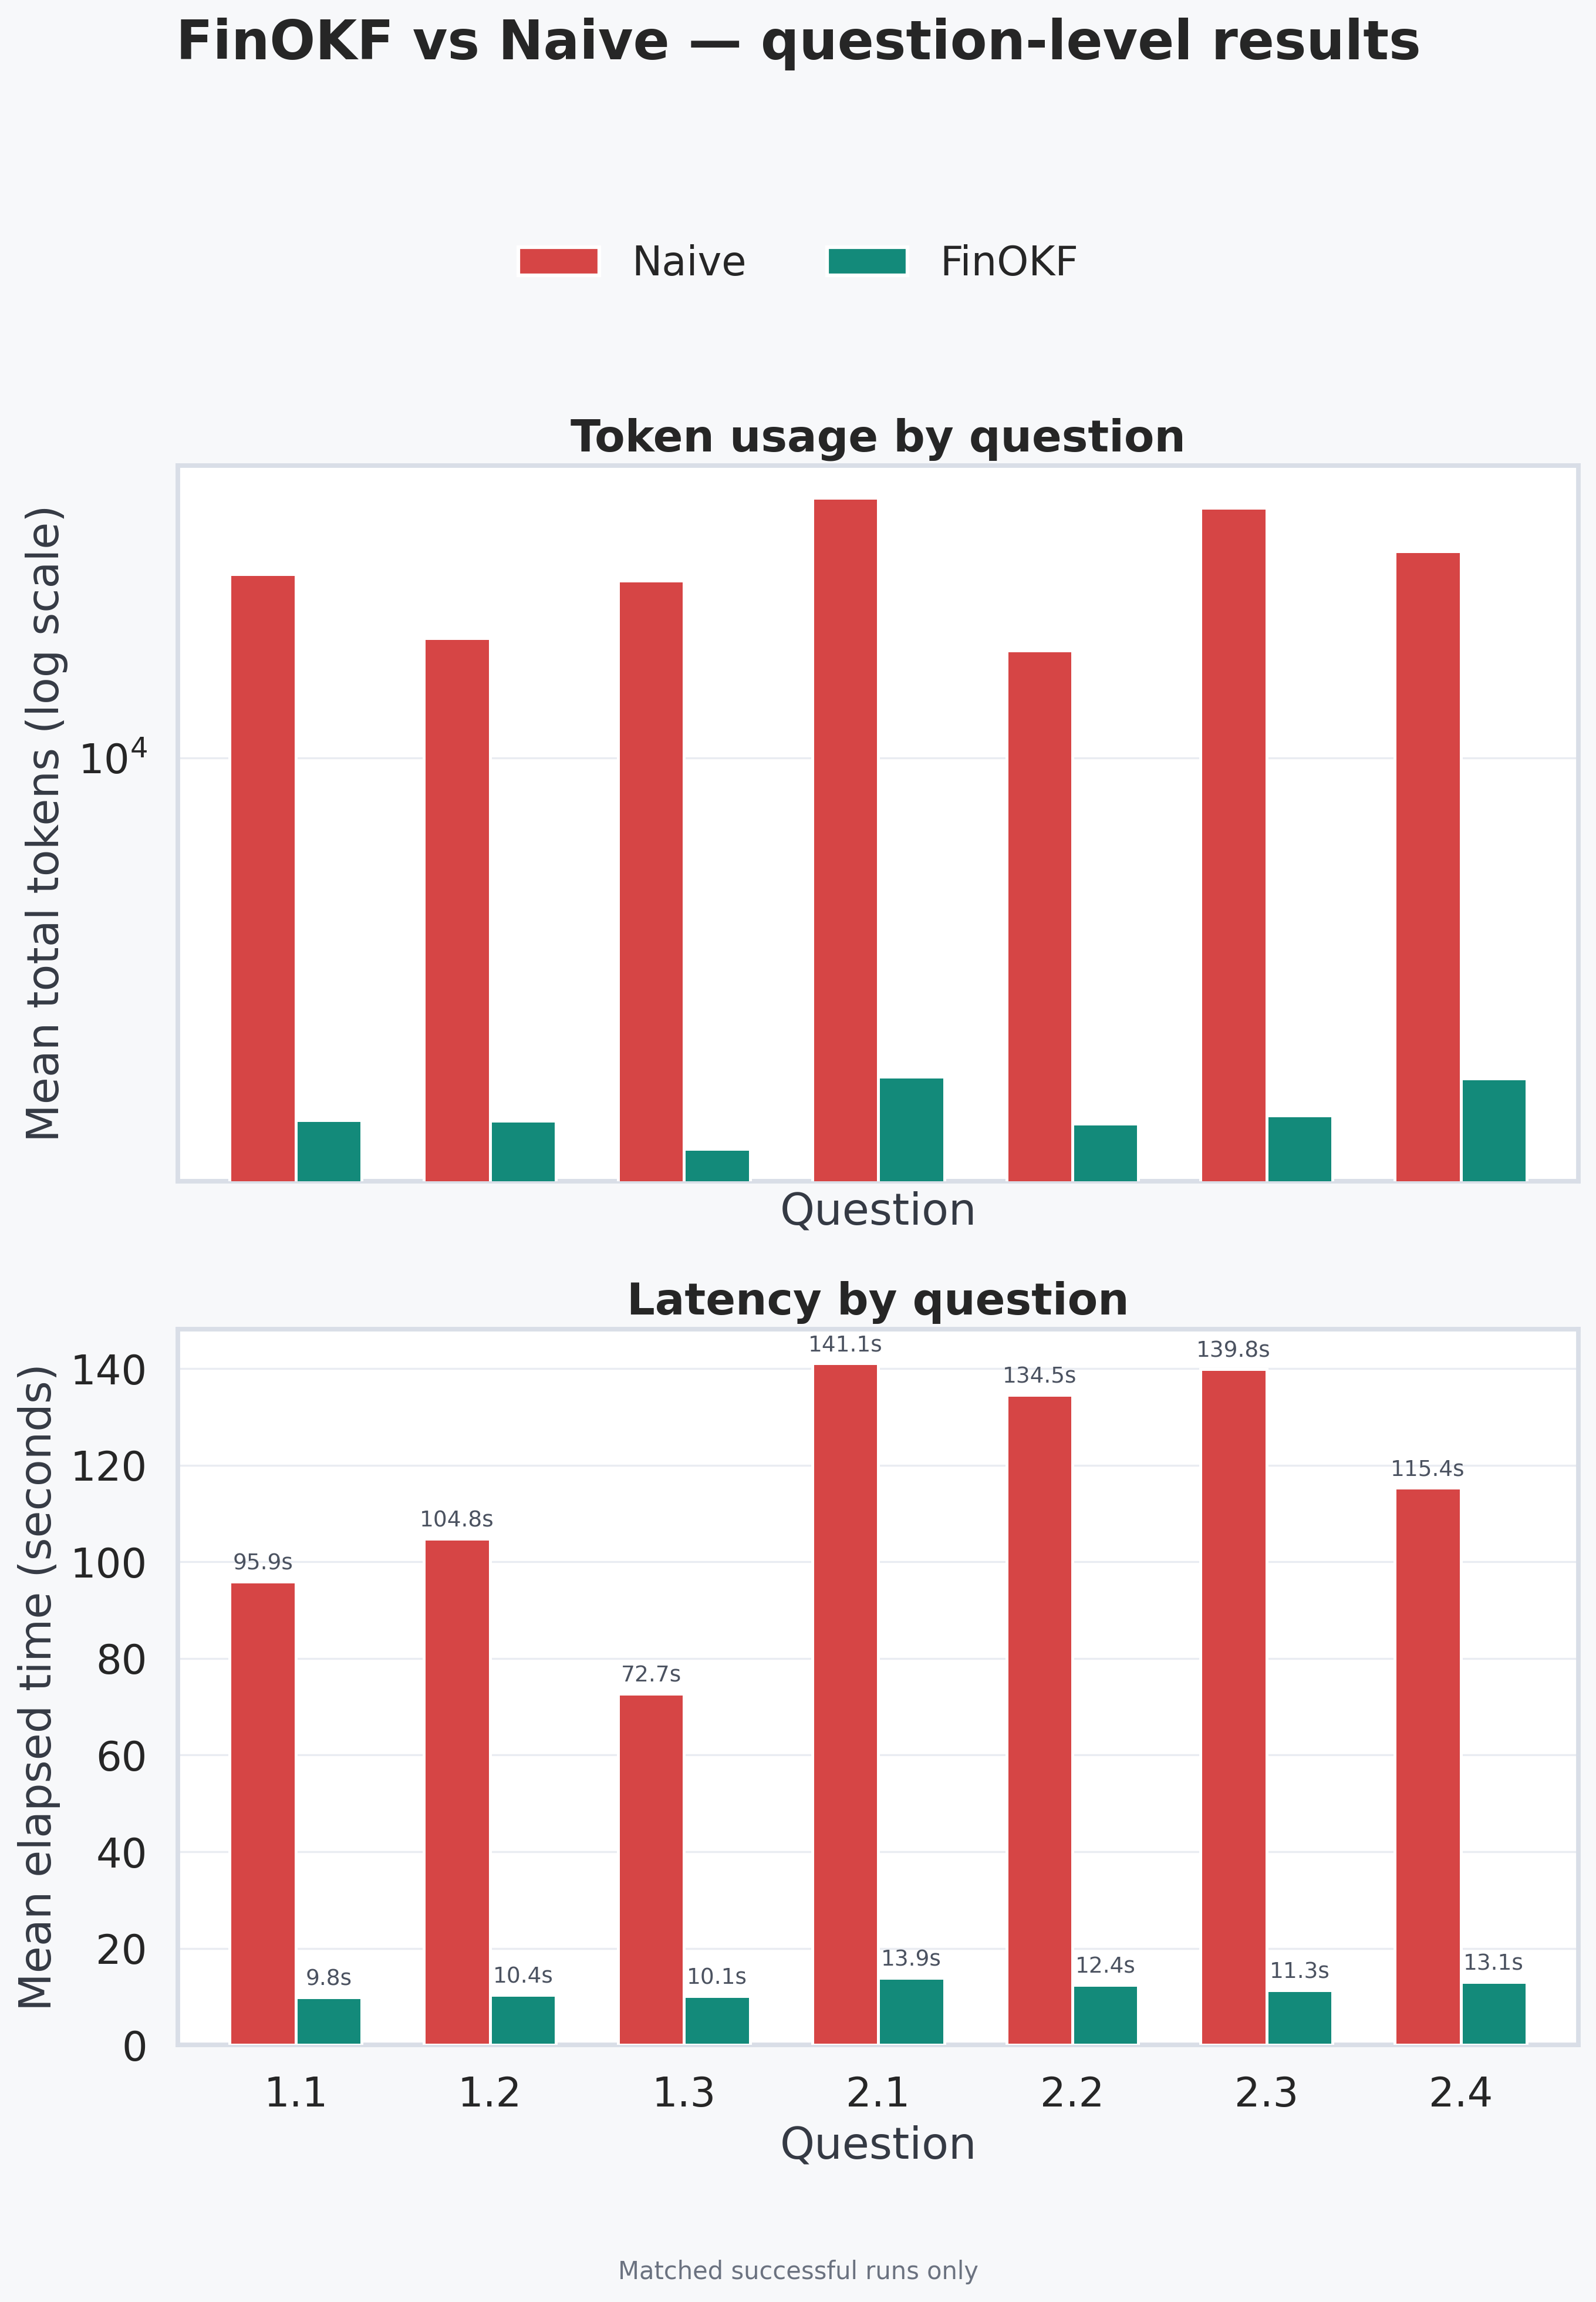
\includegraphics[width=0.92\columnwidth,height=0.42\textheight,keepaspectratio]{../assets/question_results_vertical.png}
\caption{Question-level costs pooled over matched configurations: three for 2.1 and 2.3; two for the others. Unequal composition limits comparisons across questions.}
\label{fig:questions}
\end{figure}

Figure~\ref{fig:questions} pools available matched models by question. Successful-status pairing excludes five failed Claude baseline runs from cost means, but retains them in the completion and accuracy accounting. The surviving Claude baseline texts are truncated, so lower or higher resource use cannot be interpreted as matched answer completeness. FinOKF's calculation path still performs fresh synthesis; model time is not zero on cache hits. The observed savings combine local-data access, preprocessing, call count, output budgets, and reuse rather than isolating LRU.

\section{Limitations and Next Evaluation}
The completed audit spans all three recorded configurations, but remains narrow: two issuers, seven related questions, 15 distinct reference values, and a retrospective reporting panel. Repeated entries are not independent accuracy trials. More complete margin reporting does not establish superior analyst usefulness; alternative definitions, unsupported causal claims, and period caveats require separate evaluation. The observed Claude and Llama defects directly rule out a blanket claim that deterministic inputs guarantee correct answers.

A stronger study should preregister tasks and scoring, blind independent analysts, and compare raw local retrieval, validated evidence with model arithmetic, deterministic calculation without caching, and the same path with caching. It should hold models and answer requirements constant, randomize order, reset cache state, include failures, and test source changes and research-cache expiration. Numerical correctness, consistency, abstention, citation support, completeness, and usefulness should be measured separately with repeated runs and uncertainty estimates.

The validator remains restricted to supported USD concepts and consolidated periods. It does not solve general accounting reconciliation or foreign-currency analysis. Cache validity depends on refreshed evidence metadata. Historical financial ratios remain analyst decision support, not autonomous investment recommendations.

\section{Conclusion}
Across GPT-5.5, Claude Sonnet 5, and Llama 3.2 3B, FinOKF lowers observed workflow cost and increases coverage of a common financial-measurement panel. The full-vault audit also exposes the remaining boundary: correct evidence and arithmetic do not ensure correct synthesis. GPT's audited reported values agree with the references; Claude and Llama illustrate narrative, period, and supplemental-arithmetic failures that a table-only score would miss. The knowledge graph and vault make these outcomes inspectable, while controlled trials are needed to establish broader benefits and isolate caching's contribution.

\nocite{patro2024financial}
\nocite{google2026okf}
\bibliography{FinOKFReferences}

\appendix
\section{Appendix: All-Model Audit Details}
\subsection{Manifest and Reproduction}
The audit includes all 42 saved result records from six vaults. Each model has one Microsoft vault (Questions 1.1--1.3) and one Apple vault (2.1--2.4). Each turn has a FinOKF and Naive result, and no answer is regenerated. The audit package records all 222 panel checks, reference rows, source-content hashes, omissions, inconsistent periods, failed-run status, selected narrative findings, 24 source-copy checks, and paired cost summaries. The complete records and scoring definitions are preserved with the submission for independent inspection.

Annotations assign each reported token to a metric and period through agent-assisted inspection. The script verifies token presence and numerical tolerance but is not an automatic semantic judge. The same panel definitions are used across configurations. For conflicting period claims, the audit does not cherry-pick the correct table and ignore contrary prose. No-text failures are marked unavailable. Selected narrative findings are examples, not an exhaustive set of hallucination labels or blinded human scores.

\subsection{Source Inputs and Reference Values}
The Microsoft FY2025 filing accession is \texttt{0000950170-25-100235}; Apple's is \texttt{0000320193-25-000079}. Microsoft's consolidated revenue and operating-income rows occur at lines 1356 and 1365 in the archived Markdown used by the reference parser. Apple's sales, cost-of-sales, and operating-income rows occur at lines 852, 856, and 862. Both tables declare millions, with descending year columns. The parser checks duplicate matching rows for consistency and computes ratios independently of backend bindings. Issuer reports corroborate the inspected inputs \citep{msft2025report,apple2025results,apple2024results}.

\begin{table}[t]
\centering
\begin{tabular}{llrrr}
\toprule
Issuer & USD millions & 2023 & 2024 & 2025\\
\midrule
MSFT & Revenue & 211,915 & 245,122 & 281,724\\
 & Op. income & 88,523 & 109,433 & 128,528\\
AAPL & Sales & 383,285 & 391,035 & 416,161\\
 & Cost of sales & 214,137 & 210,352 & 220,960\\
 & Op. income & 114,301 & 123,216 & 133,050\\
\bottomrule
\end{tabular}
\caption{Consolidated source inputs for every model's audit.}
\label{tab:inputs}
\end{table}

\begin{table}[t]
\centering
\begin{tabular}{llrr}
\toprule
Issuer & Metric & FY & Reference\\
\midrule
MSFT & OM (\%) & 2023 & 41.772881\\
 & OM (\%) & 2024 & 44.644300\\
 & OM (\%) & 2025 & 45.621956\\
 & IOM (\%) & 2024 & 62.968651\\
 & IOM (\%) & 2025 & 52.169280\\
 & OM change (bp) & 2024 & 287.141894\\
 & OM change (bp) & 2025 & 97.765667\\
AAPL & GM (\%) & 2023 & 44.131130\\
 & GM (\%) & 2024 & 46.206350\\
 & GM (\%) & 2025 & 46.905164\\
 & GM change (bp) & 2024 & 207.522024\\
 & GM change (bp) & 2025 & 69.881429\\
 & OM (\%) & 2025 & 31.970800\\
 & OM change (bp) & 2025 & 46.057689\\
 & IOM (\%) & 2025 & 39.138741\\
\bottomrule
\end{tabular}
\caption{The 15 distinct derived references, rounded here to six decimals. IOM and changes compare each listed year with the preceding fiscal year.}
\label{tab:gold}
\end{table}

Microsoft's three-year questions use three OM levels, two IOM values, and two OM changes; its narrowed question uses the last two levels and latest changes. Apple's three-year questions use three GM levels and two changes; its narrowed question uses the last two levels and latest change. The comparison uses each company's FY2025 OM, latest OM change, and latest IOM. This panel is explicit reporting coverage, not a complete task-success rubric.

A reported 45.62\% has tolerance 0.005 percentage points; 45.6\% has tolerance 0.05. A 2.08 percentage-point change has tolerance 0.5 bp after conversion; an integer 70 bp has the same tolerance. Claude's 46.90\% differs from 46.905164\% by 0.005164 percentage points, just outside the declared tolerance; the error is small and is not presented as a material investment error. Its associated 69 bp differs by 0.881429 bp, also outside tolerance. The script retains exact errors for sensitivity analysis.

\begin{table}[t]
\centering
\begin{tabular}{llrrrrrr}
\toprule
Model & Q & \multicolumn{3}{c}{FinOKF} & \multicolumn{3}{c}{Naive}\\
 & & C & E & O & C & E & O\\
\midrule
GPT-5.5 & 1.1 & 7 & 0 & 0 & 5 & 0 & 2\\
GPT-5.5 & 1.2 & 7 & 0 & 0 & 1 & 0 & 6\\
GPT-5.5 & 1.3 & 4 & 0 & 0 & 4 & 0 & 0\\
GPT-5.5 & 2.1 & 5 & 0 & 0 & 5 & 0 & 0\\
GPT-5.5 & 2.2 & 5 & 0 & 0 & 0 & 0 & 5\\
GPT-5.5 & 2.3 & 3 & 0 & 0 & 3 & 0 & 0\\
GPT-5.5 & 2.4 & 6 & 0 & 0 & 4 & 0 & 2\\
Claude & 1.1 & 7 & 0 & 0 & -- & -- & --\\
Claude & 1.2 & 4 & 0 & 3 & -- & -- & --\\
Claude & 1.3 & 4 & 0 & 0 & -- & -- & --\\
Claude & 2.1 & 5 & 0 & 0 & 1 & 2 & 2\\
Claude & 2.2 & 5 & 0 & 0 & -- & -- & --\\
Claude & 2.3 & 3 & 0 & 0 & 3 & 0 & 0\\
Claude & 2.4 & 6 & 0 & 0 & -- & -- & --\\
Llama & 1.1 & 7 & 0 & 0 & 0 & 0 & 7\\
Llama & 1.2 & 6 & 1 & 0 & 0 & 1 & 6\\
Llama & 1.3 & 4 & 0 & 0 & 0 & 0 & 4\\
Llama & 2.1 & 5 & 0 & 0 & 0 & 0 & 5\\
Llama & 2.2 & 3 & 2 & 0 & 0 & 0 & 5\\
Llama & 2.3 & 3 & 0 & 0 & 0 & 0 & 3\\
Llama & 2.4 & 4 & 0 & 2 & 0 & 0 & 6\\
\bottomrule
\end{tabular}

\caption{Per-question audit. C: correct; E: incorrect or inconsistent; O: omitted. Dashes denote a no-text failed execution, not an omission or zero cost. All models use the same per-question denominator.}
\label{tab:question-audit}
\end{table}

\subsection{GPT-5.5 Case Analysis}
Both agents supply correct reported panel values. FinOKF covers all 37 entries. Naive's 15 omissions comprise two Microsoft initial margin changes; six quantities in its Microsoft follow-up; all five Apple repeated-question entries; and two IOM entries in the comparison. The Microsoft follow-up nevertheless draws the correct fading-leverage conclusion from rounded growth rates. Apple's repeat explicitly abstains because the answer reports insufficient fetched evidence. These responses distinguish useful qualitative reporting and safe abstention from numerical fabrication.

The comparison uses different valid leverage measures:
\begin{equation}
L=\frac{\Delta O/O_{2024}}{\Delta R/R_{2024}}
 =\frac{\mathrm{IOM}}{\mathrm{OM}_{2024}}.
\end{equation}
Apple can have higher growth-rate leverage $L$ while Microsoft has higher IOM, because their starting margins differ. We record missing IOM entries without calling Naive's alternative ranking an error. Naive explicitly flags the noncoterminous fiscal periods; FinOKF omits that caveat. No claim of general GPT answer perfection follows from the numerical panel.

\subsection{Claude Sonnet 5 Case Analysis}
FinOKF's three omitted entries are the annual OM levels in Question 1.2; all 34 reported panel entries pass. However, the same answer calls the 62.97\% to 52.17\% IOM decline nearly halving; the relative fall is about 17.2\%. Question 1.3 says operating income grows faster in absolute terms, although revenue increases \$36,602 million versus operating income's \$19,095 million. Operating income grows faster proportionally. Both are interpretive errors despite correct source values.

Apple's initial answer states a two-year gain of 278 bp; the unrounded value is 277.403453 bp, which rounds to 277 at integer precision. This supplemental value is outside the fixed annual-change panel and is explicitly reported as an additional rounding defect. The repeated answer proposes an FY2026 margin assumption near 46--47\%, unsupported by the ratio-only evidence. The narrowed answer states 4.9\% cost growth in prose but 5.0\% in its table; the source calculation is approximately 5.043\%. The company comparison first reverses an inequality, then explicitly corrects itself. That correction is retained as a presentation defect rather than an uncorrected panel-number failure.

Five Naive records report \emph{Anthropic returned no text output.} These are observed failures, not inferred from missing CSV rows. The two successful-status responses are incomplete: Question 2.1 ends during a services-cost expression and 2.3 during a services-revenue statement. They supply six panel entries, four correct and two rounding failures, leaving two omitted and 29 unavailable across failed executions. Question 2.3 also attributes the consolidated improvement entirely to mix; the exclusive causal claim is not established by the aggregate comparison. Successful-status cost means must be read alongside this incompleteness.

\subsection{Llama 3.2 3B Case Analysis}
The FinOKF Microsoft repeat assigns 62.97\% IOM to FY2023 and 52.17\% to FY2024, shifting the first interval and introducing a wrong FY2024 entry. The latest FY2025 value remains correct. The Apple repeat supplies correct interval labels in the table but shifts both gains one year early in its conclusion; both affected entries are inconsistent. The comparison omits two IOM quantities. These yield 32 correct, one incorrect, two inconsistent, and two omitted panel entries.

Numerical tables do not capture all defects. The narrowed Microsoft answer says 45.62\% is lower than 44.64\%. Apple's initial answer says annual margin gains are strengthening even though they fall from 207.5 to 69.9 bp. It also reports a 6.8\% FY2024 cost decline instead of approximately 1.77\%, and a 5.4\% FY2025 decline instead of approximately 5.04\% growth. The narrowed Apple answer attributes improvement to pricing and efficiency before conceding that the cause is not stated. The comparison labels $\Delta O/\Delta R$ as the change in operating margin, conflating IOM and margin expansion.

Naive's Microsoft repeat misassigns FY2025 revenue and income to FY2024, producing the sole explicit panel entry, an incorrect 45.6\% FY2024 margin. Its narrowed answer gives \$130.8 billion FY2025 operating income instead of \$128.528 billion. Apple's initial and repeated answers substitute quarterly gross-profit amounts for annual analysis, with the repeat inventing a \$43,427 million prior-quarter amount. The narrowed answer converts \$48,341 million into 48.341\% without dividing by sales. The comparison uses gross margin divided by revenue as operating leverage. Thus the 36 omitted annual panel entries conceal additional errors outside the panel; they do not mean the answers safely abstained on all those topics.

\subsection{Audit Boundaries}
All six vaults are included in status and accuracy accounting; cost pairing excludes failed statuses symmetrically by question and model. Reference measurements remain shared across models, so neither 222 checks nor 111 entries per agent are independent accuracy trials. There are no blinded raters, inter-rater statistics, exhaustive narrative labels, or analyst-usefulness scores. The selected defects are tied to exact saved text and verifiable source arithmetic, but they are not a complete error taxonomy.

The 24 source-copy checks concern metadata-recorded local filing sources. They do not establish correctness of every displayed citation, eliminate preprocessing risk, or prove support for causal claims. In particular, some Llama answers refer to price or CSV evidence beyond those source records. The corpus and conversation graphs support inspection of such discrepancies; they do not prevent the model from creating them.
\end{document}
